\documentclass{article}

\usepackage{tikz}
\usepackage{graphicx}
\graphicspath{ {./figures/} }

\title{Personal Issue Tracker Proposal}
\author{ATeam-30}

\begin{document}

\maketitle

\textbf{Contributors:}

James Charapata: jcharapata@wisc.edu

Martin Diges: mdiges@wisc.edu

Tyler Johnston: tjjohnston2@wisc.edu, tjohnston@cs.wisc.edu

Mingrui Leng: mleng2@wisc.edu

Alec Lowry: lowry3@wisc.edu


\tableofcontents
\newpage

\section{Problem}

    The goal of this product is to offer a comprehensive tool for tracking issues and features to be implemented.
    Will compliment git version control for easy tracking of the development and implementation process.
    In addition, it will allow for easy handling of issues that pop up throughout the development process.

\section{Primary Stakeholder}

    Primarily designed with software development in mind, but could be used for most projects in the development and maintenance phase.

\section{Graphical User interface}

    Upon application launch, IssueTracker initializes to a screen representing all current projects and issues (figure 1). Figure 2 represents a sample screen for the creation of a new issue.

    \fbox{ 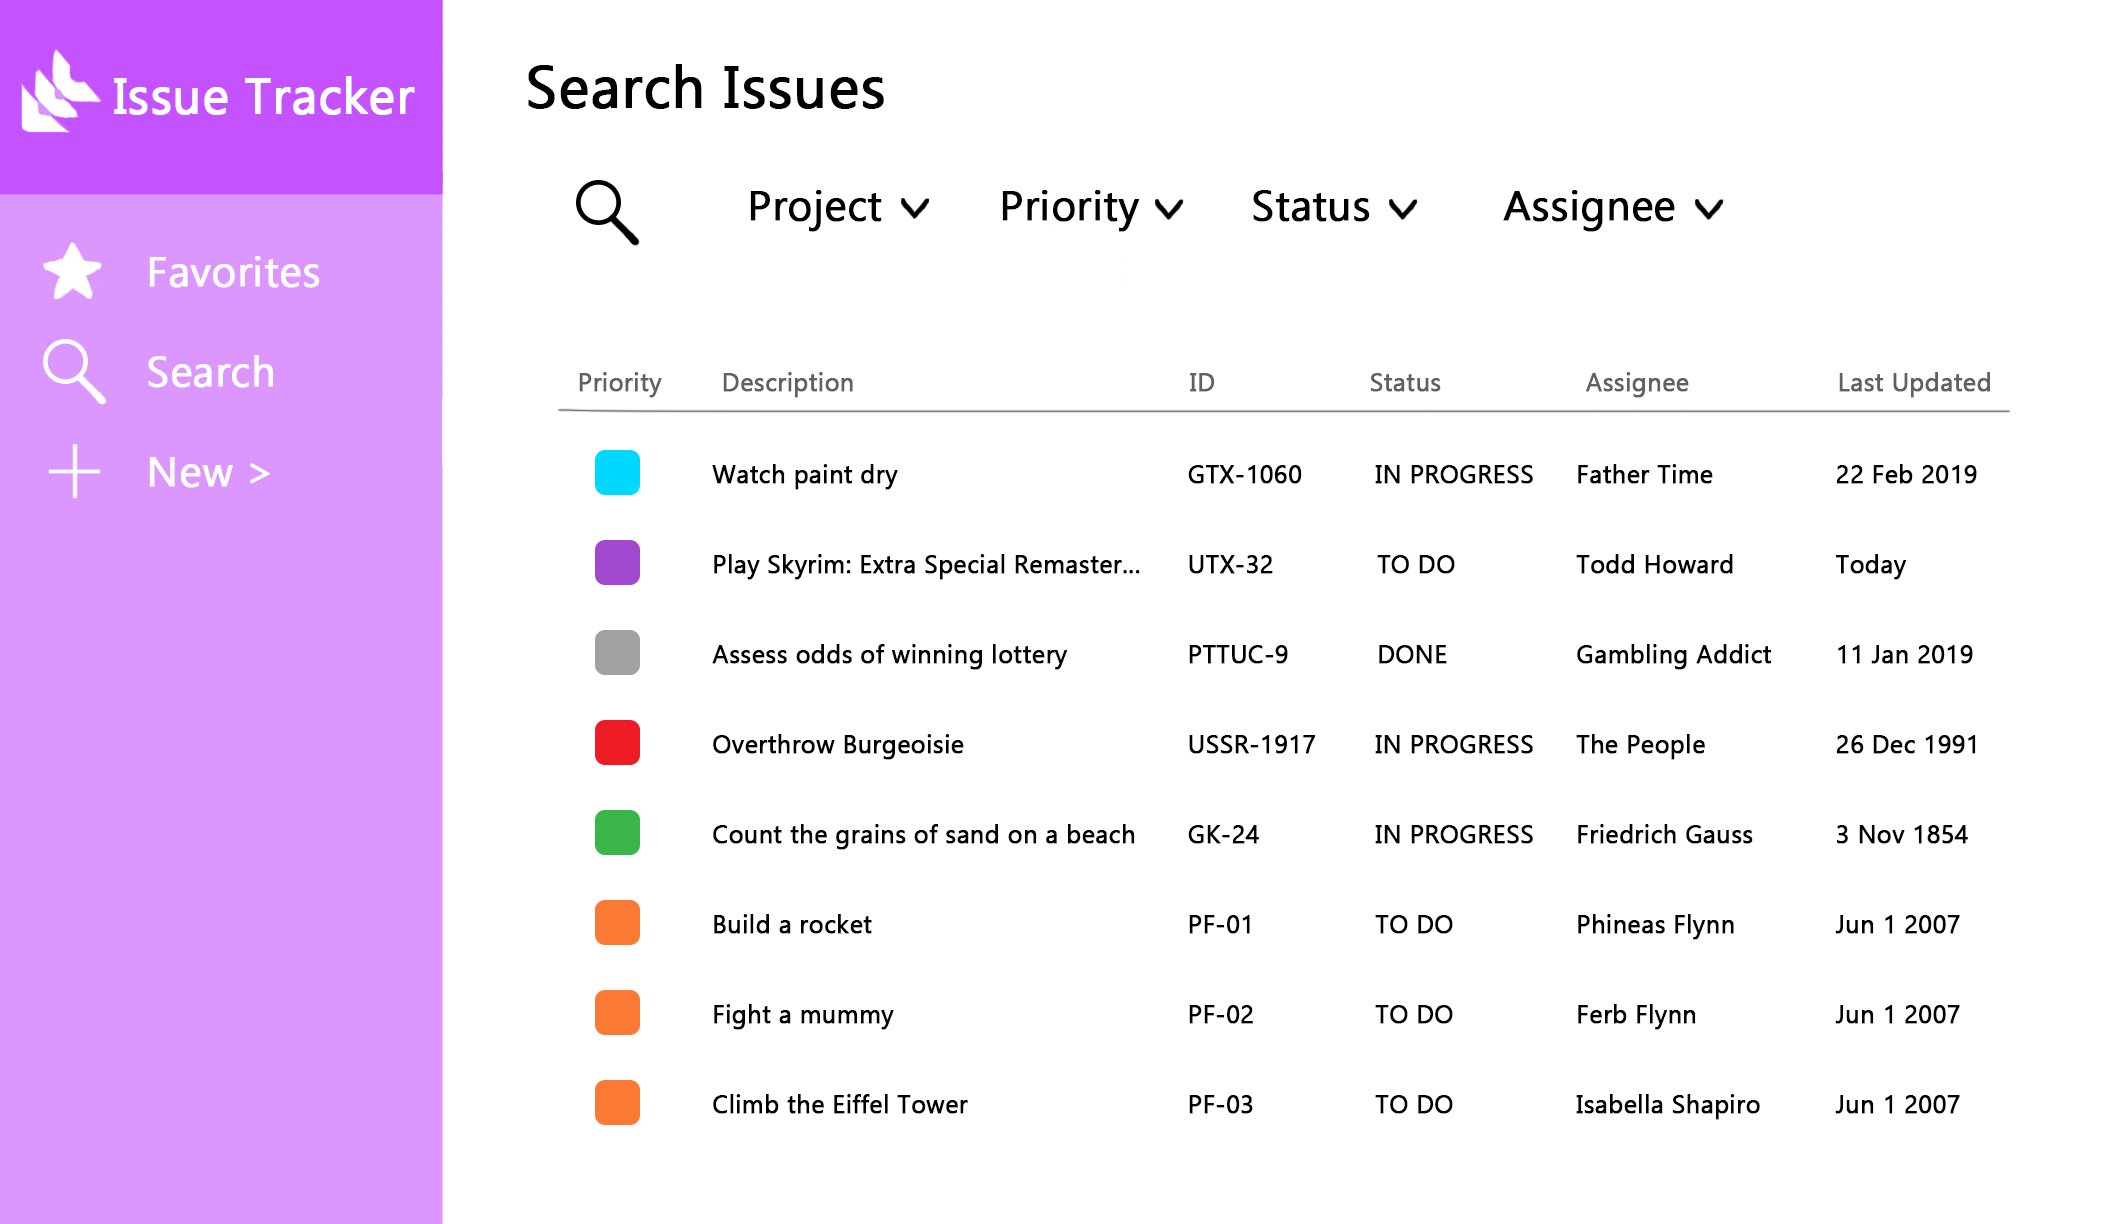
\includegraphics[scale=0.175]{IssueTrackerGUI_IssueList.png} }
    \fbox{ 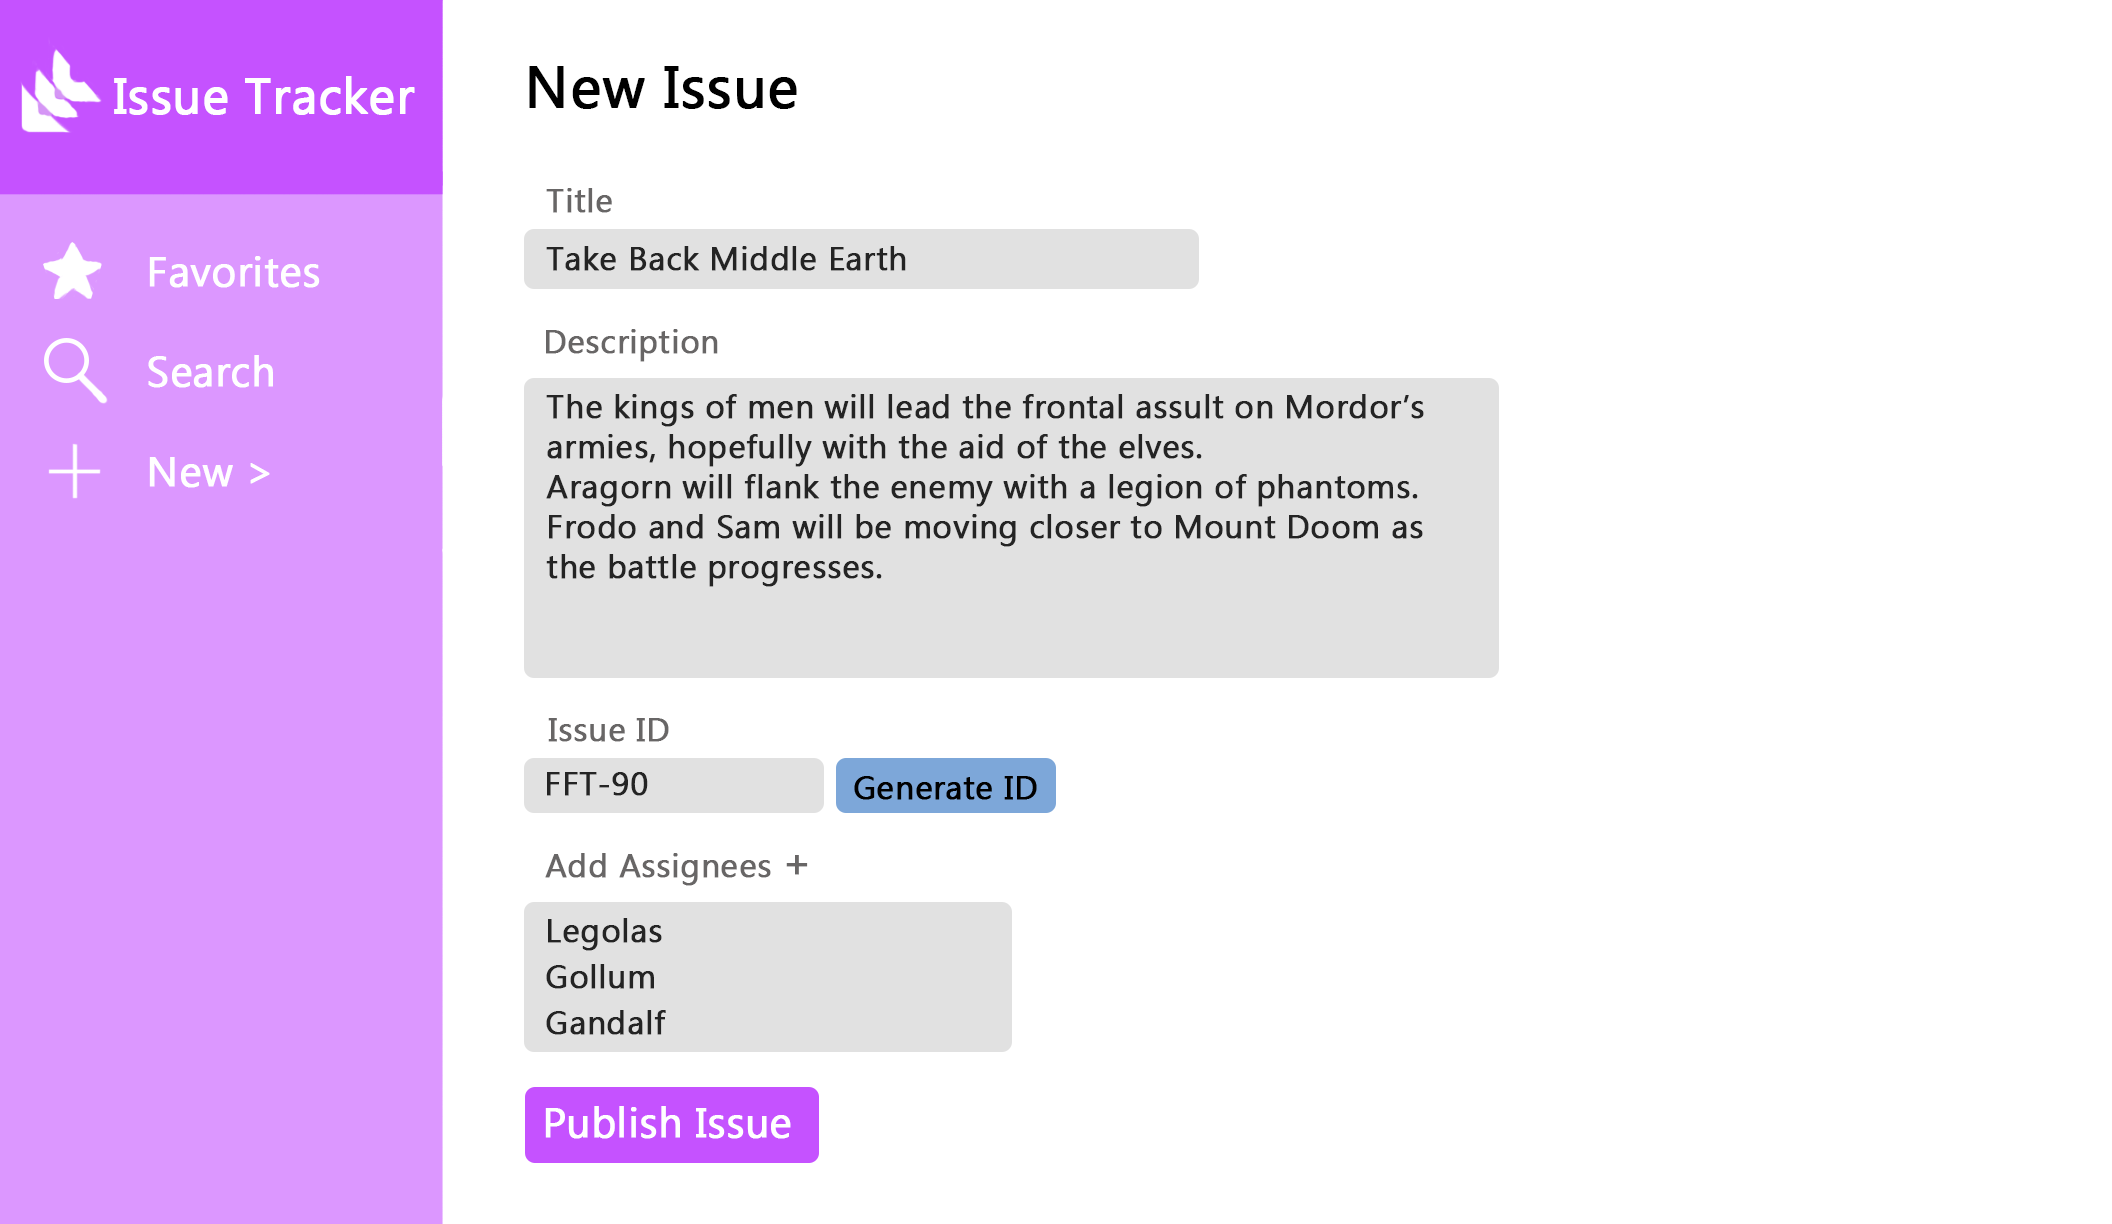
\includegraphics[scale=0.175]{IssueTrackerGUI_NewIssue.png} }

\section{Data Structure}

    \fbox{ 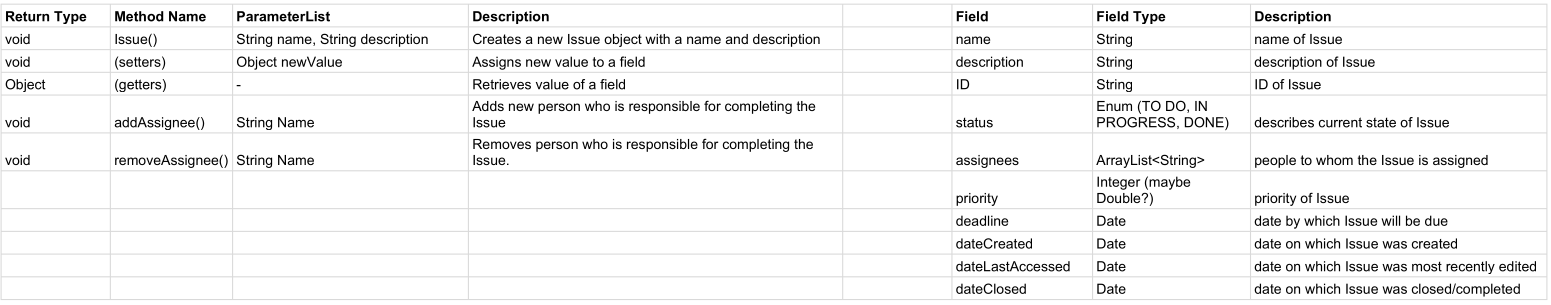
\includegraphics[scale=0.35]{ClassTable_Issue.png} }
    \fbox{ 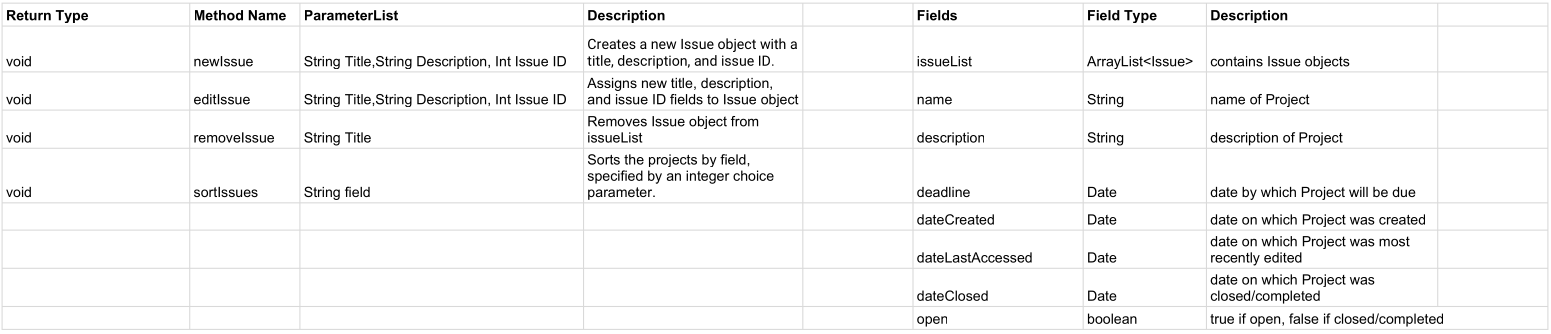
\includegraphics[scale=0.35]{ClassTable_Project.png} }
    \fbox{ 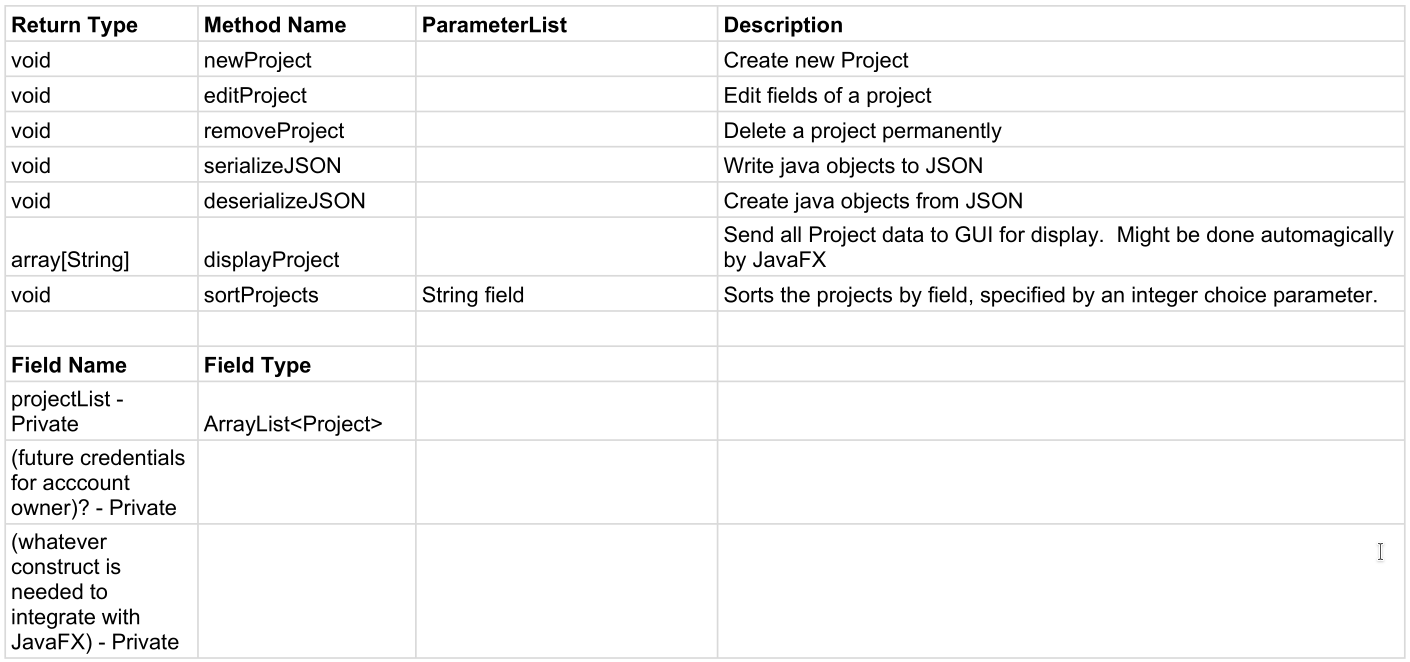
\includegraphics[scale=0.4]{ClassTable_IssueTracker.png} }

\section{Object Diagram}

    \fbox{ 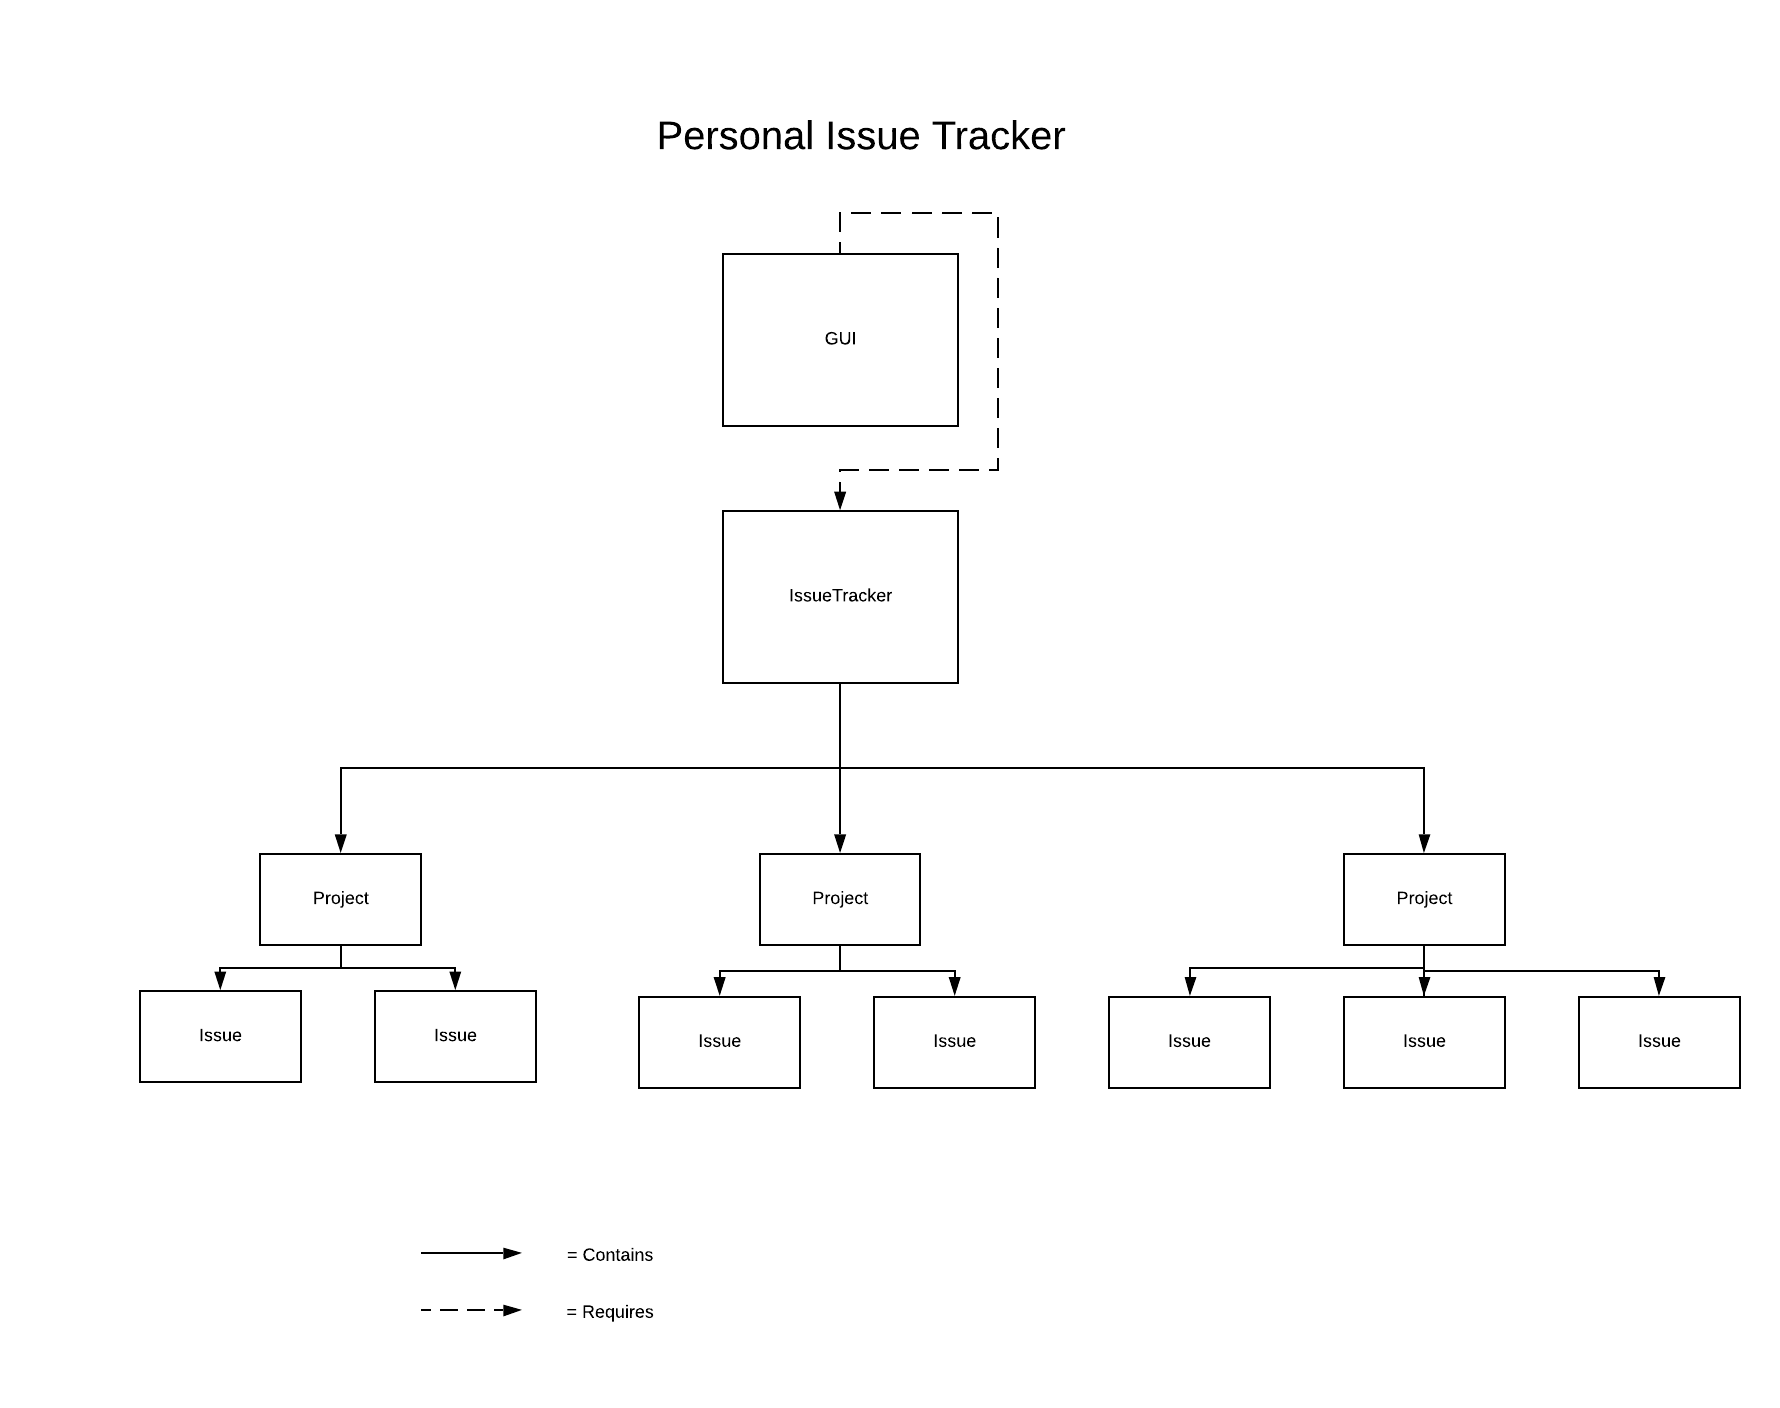
\includegraphics[scale=0.5]{ObjectDiagram.png} }

\end{document}
